\documentclass[WHATMANUAL.tex]{subfiles}

\begin{document}

\chapter{Water-level time-series preparation}\label{chap:wlvl_formatting}

The process of validation, correcting and updating water-level dataset is not very much complicated, but can represent a fastitious task, especially if there is multiple well installed in the area of study.

WHAT try to alleviate this process by providing tools to easily explore, manipulate and correct the data in a convivial dynamical graphical environment.

WHAT provides a dynamic graphical environment to explore, validate and apply various corrections to water-level time series. This feature is available in the mode ``computation'' of the tab \emph{Hydrograph} shown in Figure~\ref{fig:tab_hydrograph_computation}.

\begin{figure}[h!]
	\centering
	\setlength{\fboxsep}{0pt}
	\fbox{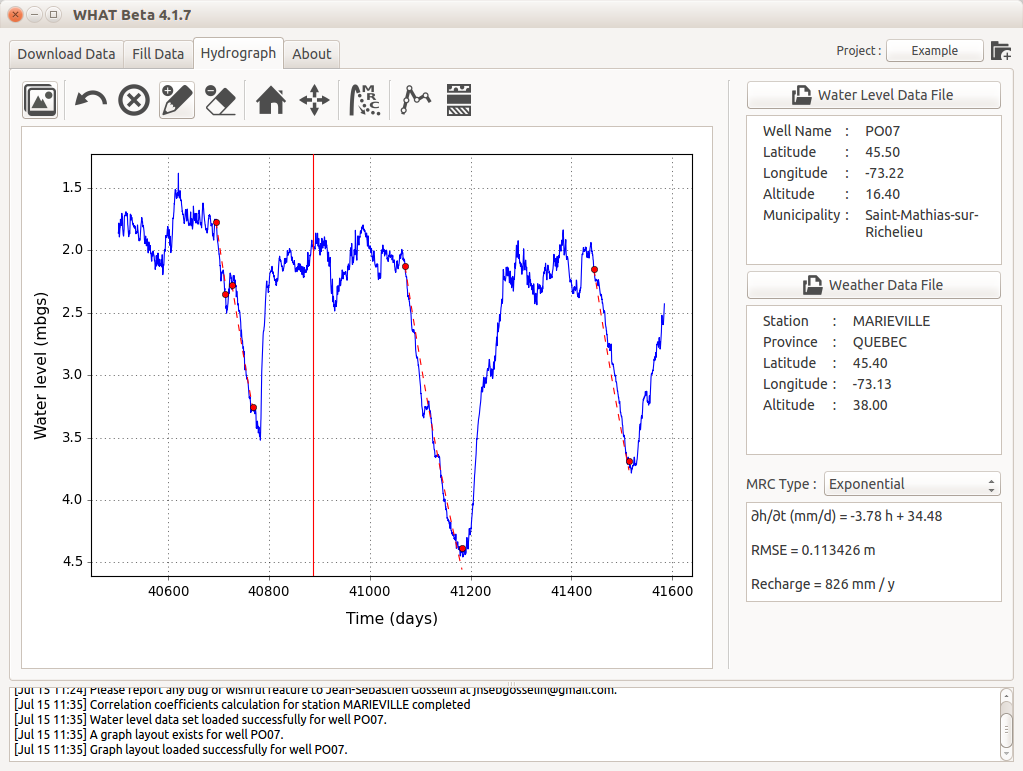
\includegraphics[width=0.75\textwidth]{img/WHAT_Screenshot003}}
	\caption[Mode ``Computation'' of the Tab ``Hydrograph''.]{Mode ``Computation'' of the Tab ``Hydrograph''.}
	\label{fig:tab_hydrograph_computation}
\end{figure}

\section{Water Level Format}

Water-level data files can be imported in either in a Microsoft Excel 2003 format (.xls) or a tab-separated values (TSV) text file (``.tsv''). A sample of a water-level data file is provided in the example that is distributed with the software. For the MS Excell format, data must be saved in the first page of the workbook, all the additional pages won't be read by WHAT for performance purposes.

%The water-levels must be entered in meters relative to the ground surface with the vertical axis being positive upward. If the depth of installation of the data logger is unknown, it is possible to estimate it with WHAT using the manual measurements if available. Otherwise, it won't be possible to exaclty position the water level in the vertical space and data. A guess estimate of the logger depth of installation can be done from the log of the well. Another alternative will be to plot the data as the height of the water column above the instrument or the submergence depth.

The water-levels must be entered as the height of the water column above the instrument or the submergence depth. This is generally directly the ouput data of vented water-level data loggers (gage pressure transducers). However, non-vented devices record the absolute pressure and their output must be compensated for barometric pressure in order to obtain a measure of the water level elevation. This is done by subtracting the barometric record from the water-level record in order to compute the height of the water column above the instrument. This correction must be made before the water-level data are loaded in WHAT. Some software by the data logger manufacturers are able to do this automatically. Alternately, this can be easily done manually when some theory basics are well understood. This is covered in more detail in Section~X of Chapter~Y.

The measurements must also be accompanied by the times, in the Microsoft Excel numeric time format, at which they were taken. The following link provides a detailed description and analysis of the numeric time format in Microsoft Excel : \url{http://www.lexicon.net/sjmachin/xlrd.html}

\section{Well Configuration and Location Information}

In addition to the data time-series, various information about the well configuration and location are required in the file header for WHAT to work properly. These information are consists in:

\paragraph{Well Name} This is an alphanumeric identifier of the well that must be unique to the project. It can contain any combination of alphabetic and numeric characters, but it is recommended to avoid using the following symbol: \%, ', ", /, \textbackslash. The Well Name is used to store various information about the water level time-series (graph layout, data modification, manual measurements, etc.) and is also used for the generation of the figure labels.

\paragraph{Latitude and Longitude} Location coordinates of the well in decimal degrees. The well location coordinates are used principally for computing the distance between the well and the weather stations and consequently for the generation of the figure labels.

There exists a great online tool for the conversion of geographic units in various format that is provided by the Montana State University. This tool can be accessed at this web address: \url{http://www.rcn.montana.edu/Resources/Converter.aspx}.

\paragraph{Altitude} Altitude of the ground surface relative to the mean see level at the well location in meters above see level. This value is used to convert the water-level measurements when the datum is changed to mean sea level.

\paragraph{Municipality} This field is currently not used in WHAT and is for informational purposes only.

\paragraph{Installation Depth} This is the fixed depth at which water-level data loggers is installed in the well or the piezometer relative to the ground surface. This value is negative if below the ground surface and positive if above.

fixed depth in a well or the piezometer from a stable fixed point called the hanging point, often secured directly to the well casing itself.

\section{Manual Measurements}

Water level manual measurements are read automatically from the file named ``waterlvl manual measurements.xls'' that is located in the project folder (see Section~\ref{subsec:folder_structure}) when a water level data file is opened in WHAT.

%\begin{sloppypar}
%\end{sloppypar}

The information are distributed in 3 columns: the unique ID of the well in which the measurement has been done, the time and the value of the manual measurement. When loading a water-level data file, WHAT will automatically search within this file for every entry that corresponds to the ID of the well. 

Manual measurements must be entered in meters relative to the ground surface with the vertical axis positive upward. Measurements below the ground surface are thus negative, and positive when above. Measurement taken relative to the casing of the well must be corrected accordingly.

It is necessary to validate the values taken with the automatic logger with manual measurement on a regular basis.

Long-term monitoring of water levels with the use of automatic data loggers can lead to errors if the data are not validated on a regular basis with manual measurements. \cite{freeman_use_2004} provides a good review on possible causes of errors that may be present in data acquired with submersible pressure transducers.

% Text cited as is. Need to reformat it.
The convenience and low maintenance of submersible pressure transducers can lead to long intervals between calibration checks and overconfidence in the reliability of the sensor's data. If checks on the calibration of sensors are not made, data may be erroneous to the point of leading to incorrect hydrologic interpretations.

\section{Loading the data and Computation mode overview}

The first step is to open the water-level data file in WHAT. This is done simply by clicking on the \emph{Water Level Data File button} that is located at the top of the right side panel of the tab \emph{Hydrograph}. This will open a new window for the selection of a valide water-level data file. Clicking on select will open the file in WHAT. The water level time-series will then automatically be loaded in WHAT and the data should be automatically plotted. If there is weather data files already present in the ``Output'' folder, the program will automatically load the file from the closest weather station to the well and will also plot the data along with the water-level measurements.

The correction and adjustment of water-level time-series is done in mode 'Computation' of the tab hydrograph. By default, this tab is opened in mode Layout. This feature will be covered in detail in Section~\ref{chap:plotting_data}. Switching from the Layout to the Computation mode is done by clicking on the button ``Toggle'' located at the left end of the toolbar. If a water-level time-series is already imported in WHAT, the data should appear in the graph located in the left pane of the window. If a weather data file has been selected, air temp. and precipitation should also appear on the graph.

The display in mode 'Computation' is dynamic, meaning that it is possible to interact directly with the graph to pan and zoom the content of the graph. By design, only the water-level can be zoomed or panned while the weather data will ajust in the time dimension but will stay static in the vertical axis. This allow a more consistent experience when trying to interpret the water-level time series. 

In order to active the dynamical capability of the graph, the button Pan\&Zoom must be toggled on in the toolbar. Panning the vertical or horizontal axes is achieved by holding the left button of the mouse and dragging the mouse horizontally or vertically. Zooming is achieved by holding the mouse right button and dragging the mouse horizontally to zoom in or out in the time axis or vertically for the vertical axis. Zooming both axes equally at the same time can be done by holding the right button and dragging the mouse at an angle of 45 degree toward or away the center of the graph for zooming in and out respectively.

\section{Water Level Corrections}

The second step is to apply corrections obtained from field verification measurements. If the record is faulty due to instrumentation or other problems, corrections usually cannot be applied. In general, a missing or faulty record of ground-water level cannot be estimated reliably.

Four types of corrections can be applied to the record:

datum corrections,
hung-depth corrections,
drift corrections,
and calibration corrections. 
Aberration value correction

When data are manipulated in WHAT, the original dataset is not altered directly. Modification are applied to a copy of the originral dataset in order to preserve the later. In addition, each modification applied to a given set of data is registered in a log file.

\subsection{Aberrant values}

Aberrant values represent water-level measurements that are not representative of the piezometric level of the aquifer in which the well is installed. These values can corresponds to measurement taken when the instrument was out of the water when downloading the data or during a test in the well, or can represent non natural behavior of the level in the well dur for example of pumping during an echantillanage test. Figure Y shows an example of an example with aberrant values that were du to measurement taken while the instrument was out of the water. Tyipically, these measurement will have a value close to zero, since the pressure measured, once corrected for barometric pressure, correspond to a water column of zero height.

These aberrant value complicate the process of interpreting the data and can be removed from the dataset. 

Aberrant value can be removed individually in the dataset. To to so, the data can be displayed as dots. The tool remove aberrant data can be used to remove the aberrant data. The process consist in clicking on the button to toggle the edition of data and to hover over the data point that is aberrant. A cross should appear on the data point. Right clicking with the mouse on the data point will remove the points from the data. It is possible to undo up to 10 operation done on the data.

\subsection{Hung-depth corrections}

Hung-depth errors are caused when the transducer changes relative to its original position, due either to purposeful or accidental raising or lowering of the transducer in the well. In a given project, there may be multiple team that may have access to the well. It is not always possible to track every visit to the well. However, it occurs frequently that the instrument is not replaced exactly at the same place in the well. This generally won't be perceptible when looking at the hydrograph using a continuous line. However, these errors become apparent when plotting each data point as individual dots. Figure Y show an example of an hydrograph where the water-level data logger was not reinstalled at the same depth in the well dur to mixed cables. The situation was corrected in a subsequent visit to the well.

These occur in the data as discontinuity the variation of the time-series. It is possible to correct these discontinuity in WHAT.

\subsection{Datum correction}

This operation consist in best-fitting the continuous, aberrant value free, water-level time-series with the manual measurement made in the well. The fit is done by translating and rotatting the curve in order to best fit the manual measurement. The translation allow the correction to any error in the estimation of the depth of installation of the instrument. In addition, if the depth of estallation was previously unknown and set to a value of zero, this will allow the estimation of the depth of installation of the instrument.

the rotating part in the correction is for the correction of any drift that could occur in the automatic measurements of the data by the data logger. The cause and theory for drift in the measurements is covered in detail in ref. 

A study of vertical hydraulic head gradients at a well nest in New Hampshire showed that uncorrected data from submersible pressure transducers resulted in an interpretation of reversals in vertical hydraulic-head gradients when none actually occurred (Rosenberry, 1990). In the New Hampshire study, linear adjustment of data based on monthly check measurements would have led to the conclusion that additional water-table fluctuations of up to 0.17 ft occurred when weekly check measurements indicated that sensor drift actually was responsible for those interpreted water-level fluctuations.

So this is a parameter to keep an eye on when doing the validation of the water level time series.

In the project Monteregie Est of the PACES project, the tolerated value for the difference between manual measurement and automatic values was of +- 5 cm.

\end{document}